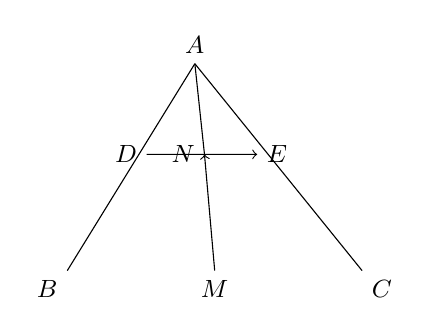
\begin{tikzpicture}[scale=.72, every node/.style={font=\small}]
  \coordinate (A) at (2.25,3.65); \coordinate (B) at (0,0);
  \coordinate (C) at (5.2,0); \coordinate (M) at (2.6,0);
  \coordinate (D) at (1.4,2.05); \coordinate (E) at (3.35,2.05);
  \coordinate (N) at (2.42,2.05);
  \draw[->] (A)--(B) (A)--(C) (D)--(E);
  \draw (A)--(N);
  \draw[->] (M)--(N);
  \foreach \p/\pos in {A/above,B/below left,C/below right,M/below,D/left,E/right,N/left}
    \node[\pos] at (\p) {$\p$};
\end{tikzpicture}
